% !TEX root=main.tex

\section{Introduction}
% Introduce the topic of multi-agent MAV networks
As Miniature Aerial Vehicles (MAVs) are becoming increasingly stable and capable agents. They have been applied in military, private and commercial enterprises in situations such as infrastructure inspection\cite{Steich2016, Ham2016}, 3D-mapping~\cite{Remondino2011}, and disaster relief\cite{Adams2011} among others.

% Talk about cooperative SLAM
As MAVs grow increasingly capable, it has become more reasonable to consider using large number of MAVs in cooperative frameworks. Many of these applications require autonomous operation in GPS-denied or GPS-degraded environments where only relative measurements to landmarks are available to provide position feedback for control and estimation.  The problem becomes further complicated as these agents must also communicate their own observations to each other to build a combined map of the environment, solve for the relative poses of the agents to one another or both. This is known as the cooperative SLAM problem.

% Introduce filter-based navigation
While cooperative SLAM has been most extensively researched in ground robots, but there have been a number of examples of cooperative SLAM on MAVs in recent literature~\cite{Loianno2015, Achtelik2012, Lawson2015}. In addition, there have been works which are marked by efforts to reduce computational requirements to perform SLAM on computationally-constrained MAV platforms with strict size, weight, and power (SWaP) requirements.  One common approach is to simplify the problem using an extended Kalman filter (EKF) to fuse interoceptive and exteroceptive sensor measurements
~\cite{Bachrach2010a, Wheeler2017b, Achtelik2009, Ahrens2009, Chowdary2013} to provide estimates of global states.

% Introduce Pose Graph optimization
One disadvantage of a global filter-based approach without global measurements is the unobservability of global position and heading states~\cite{Martinelli2012,Weiss2012,Jones2007} This causes two primary problems: global drift and inconsistency in state estimates and sub-optimal sensor fusion~\cite{Bailey2006Consistency,Bar-Shalom2002}. To correct drift, a common approach is to frame the the global trajectory as a pose graph and incorporate loop closure constraints.  The global state is then found by optimizing over poses to remove accumulated drift.  However, filter inconsistency has continued to be a documented problem in global filter-based approaches.

% Introduce relative navigation framework
Wheeler et al.~\cite{Wheeler2017a} shows that framing the navigation problem into a relative context can side-step state unobservability by directly measuring and controlling states with respect to observable landmarks.  Global states are then solely estimated with higher-order methods such as pose-graph optimization and are not in real-time feedback control loops.  This method has been shown to improve estimator performance both in simulation and in hardware experiments~\cite{Wheeler2017a, Wheeler2017b}.

% Connect relative Navigation and pose graph optimization
In the relative state estimation framework~\cite{Koch2017}, states are estimated with respect to a locally-observable ``keyframe'' image or laser scan.  As this keyframe goes out of view, another is declared and global position and heading states are reset to zero.  Uncertainty of these states is also reset to zero, as they are defined with respect to that keyframe, which is known with absolute certainty at the time of the reset.  The reset step in the relative estimator provides a clear mechanism to create mutually independent edge constraints for a pose graph.  Prior to the incorporation of loop closures, the vehicle's global pose can be calculated by traversing from the origin of the graph to the current keyframe, compounding edge constraints and finally adding the relative state.  Uncertainty in these states can be calculated using higher order methods such as those described by Barfoot et al. in ~\cite{Barfoot2014}.  After loop closures, global states can be calculated using pose-graph optimization techniques such as g$^2$o~\cite{Kummerle2011}, or iSAM2~\cite{Kaess2012}.  See Figure~\ref{fig:pose_graph} for an illustration of a pose graph.

\begin{figure}
  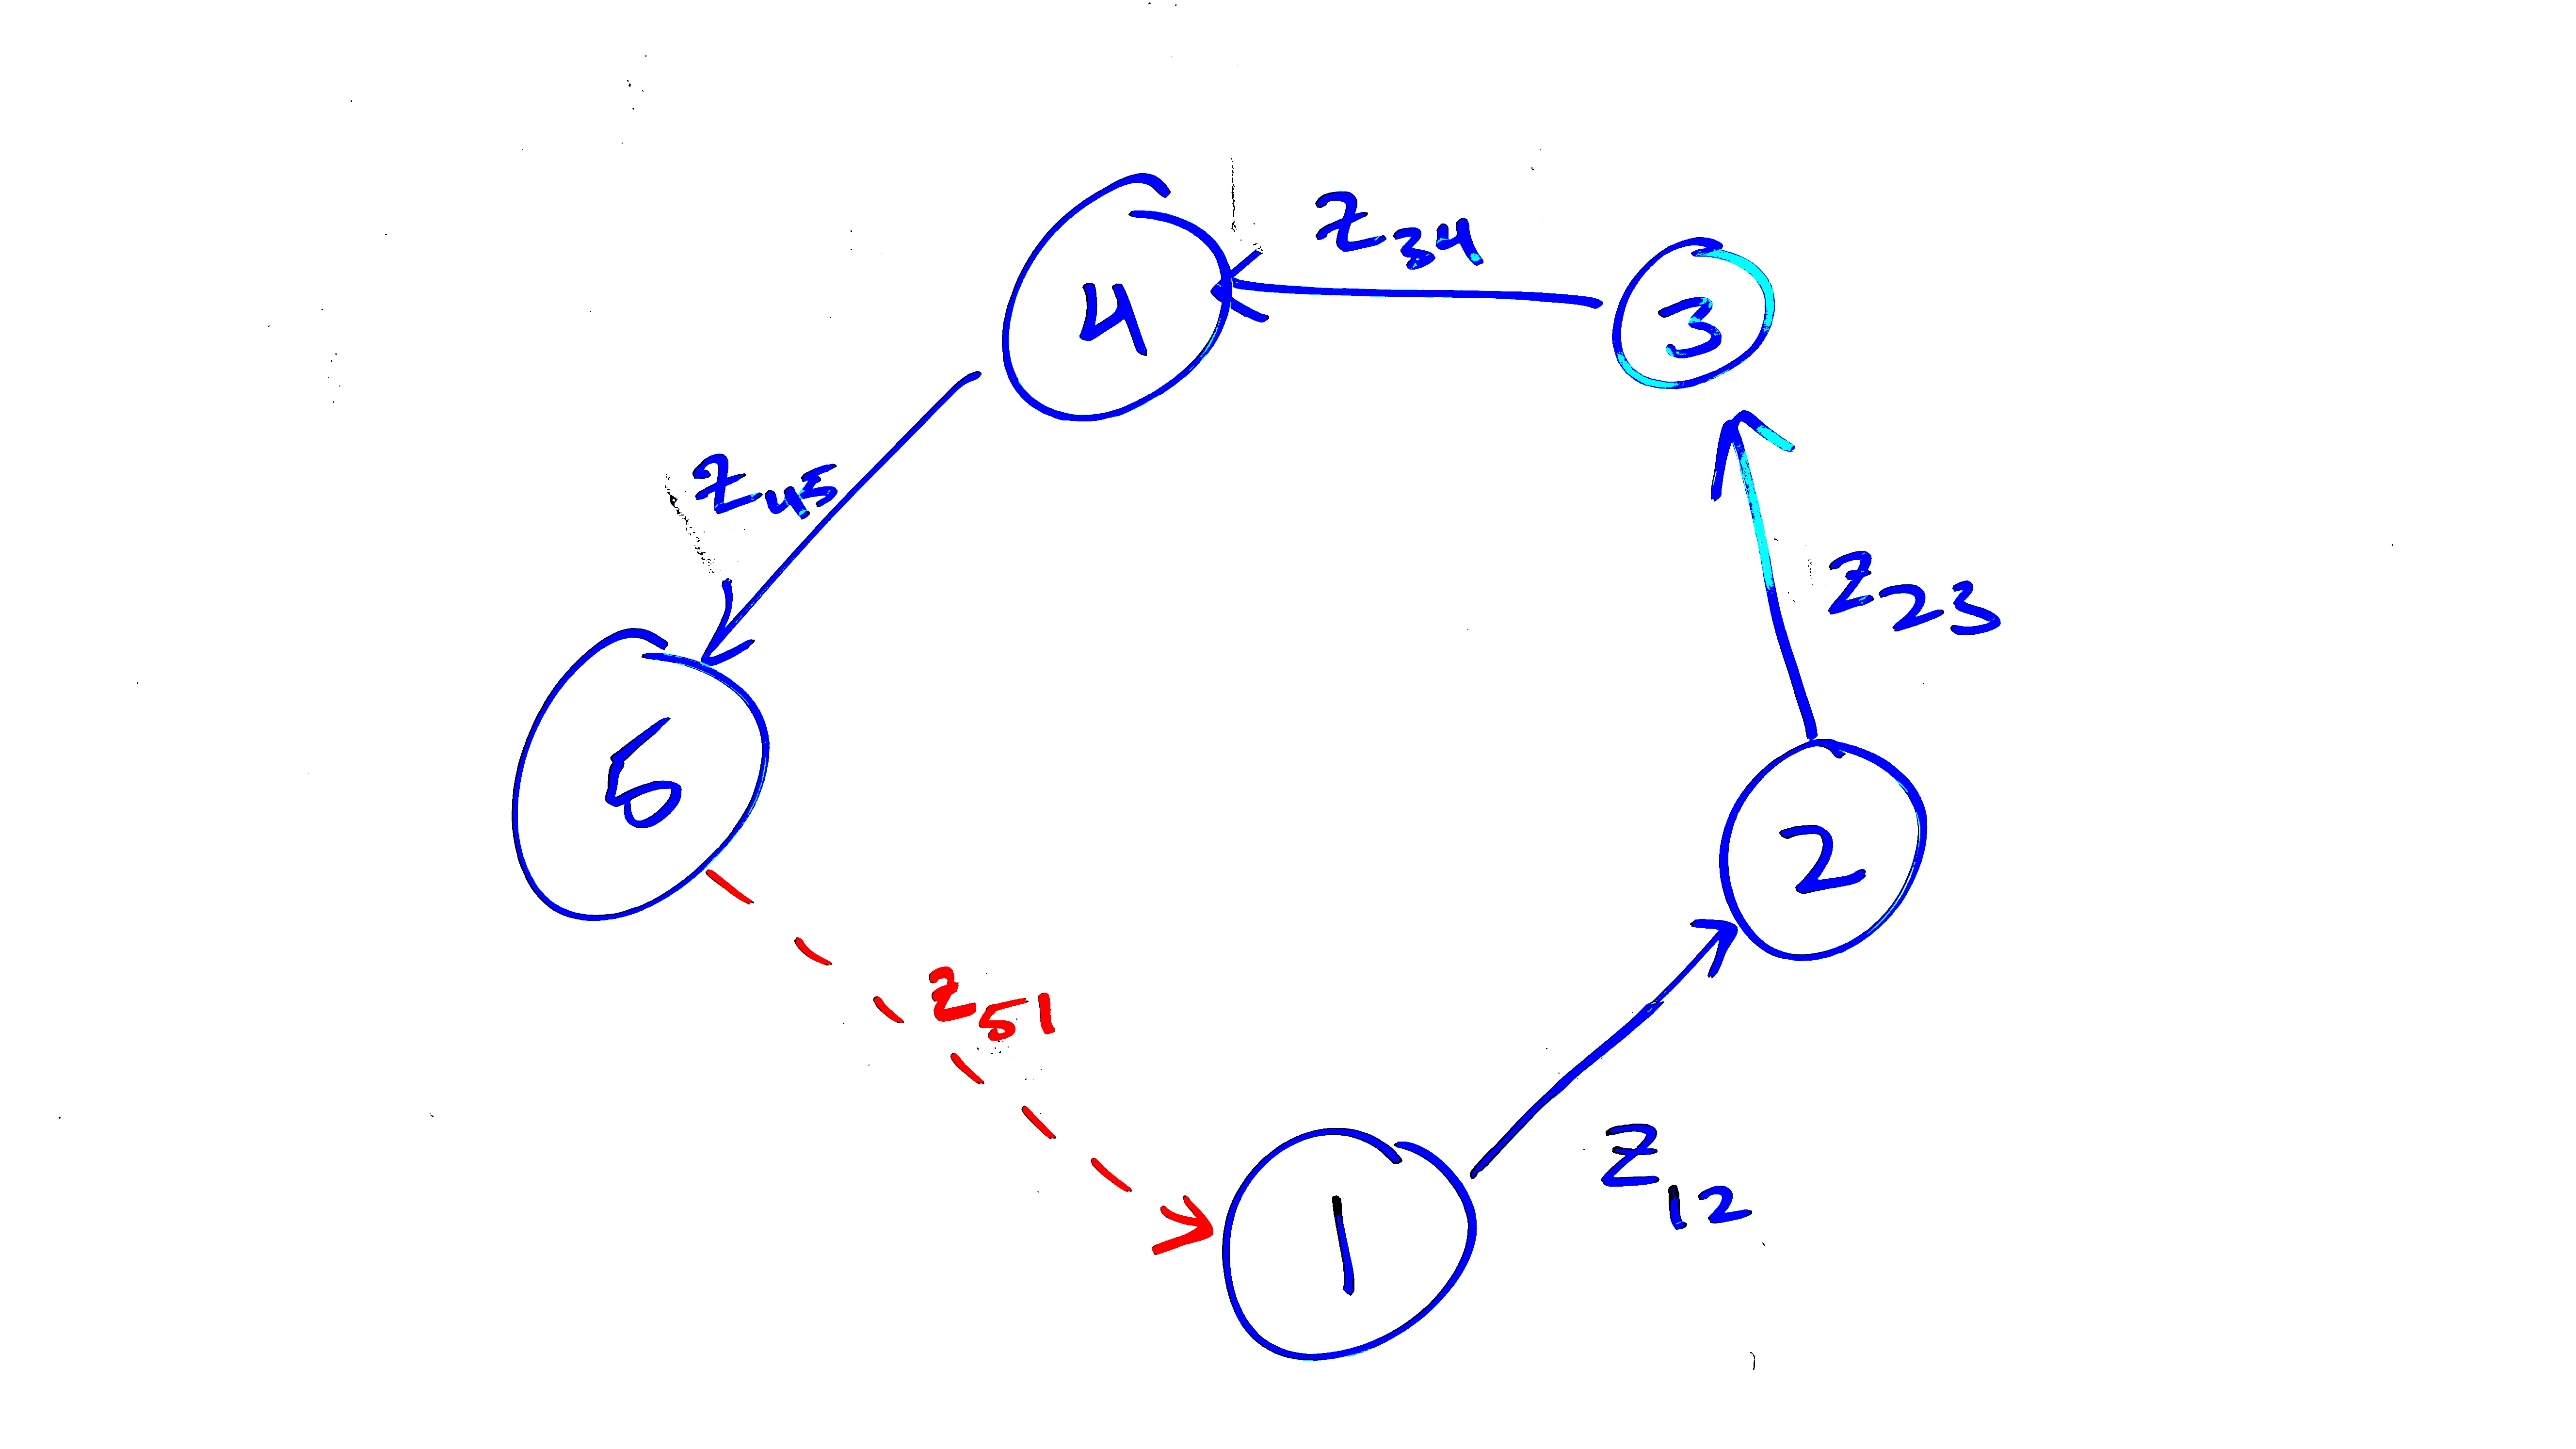
\includegraphics[width=0.7\textwidth]{figures/pose_graph.jpg}
  \caption{Illustration of a typical pose graph with a single loop closure}
  \label{fig:pose_graph}
\end{figure}

% Illustrate the idea of multi-agent relative navigation
In this work, we show the multi-agent extension to relative navigation.  Because all agents using a relative estimator navigate with respect to locally-observable landmarks, real-time control is insulated from global state updates.  This means that global states can be initialized arbitrarily and experience large updates without negative consequences on real-time performance. Additionally, as the entire map is defined in terms of mutually independent relative constraints, fusing multiple maps becomes relatively trivial.  In this work, we will show the scalability of an entirely relative multi-agent system by fusing maps from over 100 agents in real time on a laptop computer.

% Introduce edge-based optimization
One drawback of global pose optimization is a strong dependence on the quality of the initialization point for the graph.  Even a small heading error in a trajectory can result in large pose errors after a long period of time.  This problem is an active area of research and there are several prominent solutions which have been proposed~\cite{Carlone2015, Kim2010a, Agarwal2014, Wang2014}.  In this work, we present a new initialization technique in which we optimize over the edge constraints in a pose graph, rather than poses in a stochastic fashion. This method is similar to SGD-MM~\cite{Wang2014}, except we use the relative states directly, as opposed to the incremental state representation, which eliminates inconsistency issues present in SGD-MM~\cite{PAPER}

% Overview of paper
In this paper, we will first derive relative edge optimization and formulate the relative edge optimization problem and discuss the strengths and weaknesses of edge optimization when compared with global pose optimization.  We will then discuss several implementation details to ensure the practicality of edge optimization. Then, we will show results of edge optimization in a large simulation framework of 100 agents.  Finally, we will show results of a hardware demonstration of four multirotor agents.
